\documentclass[14pt]{extarticle}
\usepackage[utf8]{inputenc}
\usepackage{polski}
\usepackage{amsmath}
\usepackage{geometry}
\usepackage{graphicx}
\usepackage{multirow}
\usepackage{float}
\usepackage{esvect}
\graphicspath{{pictures/}}
\geometry{margin=0.7in}
\def\tytul{Zasada zachowania energii}

\begin{document}
\begin{table}[H]
    \centering
    \resizebox{\textwidth}{!}{
    \begin{tabular}{|c|c|c|}
    \hline
    
    \begin{tabular}[c]{@{}c@{}}Byczko Maciej\\Maziec Michał\\Pomarański Maciej\end{tabular}&
    \begin{tabular}[c]{@{}c@{}}Prowadzący:\\ dr inż. Ewa Frączek\end{tabular} &
    \begin{tabular}[c]{@{}c@{}}Numer ćwiczeń\\
    %----------------------------------------
         %<<<tutaj wpisz numer ćwiczenia
    %----------------------------------------
    \end{tabular} \\ \hline
    \begin{tabular}[c]{@{}c@{}}Grupa\\
    %----------------------------------------
        C %<<<tutaj wpisz numer grupy
    %----------------------------------------    
    \end{tabular} & \begin{tabular}[c]{@{}c@{}}Temat ćwiczenia:\\\tytul
    \end{tabular} &3\\ \hline\begin{tabular}[c]{@{}c@{}}Tydzień parzysty\\ Godzina 11:15-13:00\end{tabular}&\begin{tabular}[c]{@{}c@{}}Data wykonania ćwiczenia:\\
    %----------------------------------------
    17 marca 2020 %<<<tutaj wpisz datę
    %----------------------------------------
    \end{tabular} &\begin{tabular}[c]{@{}c@{}}Kod grupy:\\E07-50d\end{tabular}\\ \hline\end{tabular}}\end{table}
    \centering
    \section{Zadanie}
    \begin{flushleft}
        Naukowcy potrzebują twojej pomocy! Chcą zbudować ze 144 sprężyn trampolinę, która ma wytrzymać uderzenie samochodu ważącego 1500kg zrzuconego z 45 metrów.
        Sprężyny mogą maksymalnie rozciągnąć się na 4,5m. w przeciwnym wypadku samochód uderzy w ziemię.
        Policz maksymalny współczynnik sprężystości \textbf{\underline{jednej}} sprężyny jaką potrzebują naukowcy.
        Przyjmij współczynnik grawitacji 10$\frac{m}{s^2}$
    \end{flushleft}
    \begin{figure}[H]
        \centering
        \includegraphics{trampolina}
        \caption{Rysunek pomocniczy}
    \end{figure}
    \clearpage
    \section{Zadanie}
    \begin{flushleft}
        Dwóch kolegów trenują z piłkami jeden z piłką tenisową o wadze $m_1$, drugi z piłką siatkową o wadze $4m_1$. Jeden z nich wpada na pomysł aby te piłki zderzyć ze sobą więc rzucają swoje piłki tak że
        pierwsza leci pod kątem $0^\circ$ względem osi x z prędkością $v_1$=2$\frac{m}{s}$a druga pod kątem $-90^\circ$ względem osi x z prędkością $v_2$=1$\frac{m}{s}$,
        następnie zderzają się i lecą dalej gdzie druga leci pod kątem $\alpha _2$=-60$^\circ$ względem osi x.
        Znajdź prędkości końcowe tych piłek.
    \end{flushleft}
    \begin{figure}[H]
        \centering
        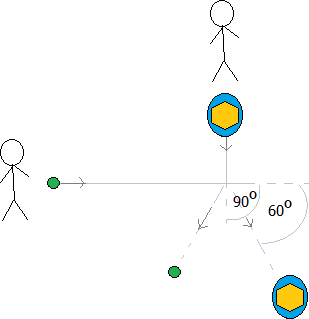
\includegraphics{pilki3p}
        \caption{Rysunek pomocniczy}
    \end{figure}
    \clearpage
    \section{Rozwiązania}
    \subsection{Zadanie 1}
    \Large
        $mgh=\frac{k_{trampoliny} \ast x^2}{2} \rightarrow k_{trampoliny}=\frac{2mgh}{x^2}$\\
        \(k_{trampoliny}=\frac{2\ast 1500 \ast 10\ast 45}{(4.5)^2} \rightarrow k_{trampoliny}=66666.(6)\frac{N}{m}\)\\
        \(k_{sprezyny}=\frac{k_{trampoliny}}{Ilosc \ sprezyn} \rightarrow k_{sprezyny}=\frac{66666.(6)}{144} = 462.(962)\frac{N}{m}\)
    \subsection{Zadanie 2}
    \large
    $m_1\vv{v_1}+m_2\vv{v_2}=m_1\vv{u_1}+m_2\vv{u_2} \rightarrow \vv{v_1} + 4\vv{v_2} = \vv{u_1} + 4\vv{u_2}$\\
    $\frac{m_1v_1^2}{2}+\frac{m_2v_2^2}{2}=\frac{m_1u_1^2}{2}+\frac{m_2u_2^2}{2} \rightarrow v_1^2 + 4v_2^2 = u_1^2 + 4u_2^2 $
    
    \begin{equation*}
        \begin{cases}
            v_1 = u_1\cos\alpha _1 + 4u_2\cos\alpha _2 &\\
            -2v_1  = u_1\sin\alpha _1 + 4u_2\sin\alpha _2 &\\
            v_1^2 + 4v_2^2 = u_1^2 + 4u_2^2  &
        \end{cases}
    \end{equation*}
    \begin{equation*}
        \begin{cases}
            \sin\alpha _1 = \frac{-2v_1+2{\sqrt{3}}u_2}{u_1}&(1)\\
            \cos\alpha _1 = \frac{v_1-2u_2}{u_1}&(2)\\
            u_1^2 = v_1^2 + v_2^2 - 4u_2^2&(3)
        \end{cases}
    \end{equation*}
    $\sin^2\alpha _1 + \cos^2\alpha _1 = 1\ \vv{z \ (1)i(2):}
    \left(\frac{-2v_1+2{\sqrt{3}}u_2}{u_1}\right)^2 + \left(\frac{v_1-2u_2}{u_1}\right)^2 = 1 \ (4)$
    \begin{equation*}
        \begin{cases}
            u_1^2 = 5v_1^2-4\left(2{\sqrt{3}}+1\right)v_1u_2+16u_2^2&(4)\\
            u_1^2 = v_1^2 + 4v_2^2 - 4u_2^2&(3)\\
            v_2 = \frac{1}{2}v_1&
        \end{cases}
    \end{equation*}
        Przyrównanie: $2v_1^2 - 4u_2^2=5v_1^2-4\left(2{\sqrt{3}}+1\right)v_1u_2+16u_2^2$\\
        $ 0 = 20u_2^2-4\left(2{\sqrt{3}}+1\right)v_1u_2+3v_1^2 $\\

        $\Delta = \left(64\sqrt{{3}}-32\right)v_1^2 $\\
        $\sqrt{{\Delta}} = 8\sqrt{{\sqrt{3}-\frac{1}{2}}} $\\
        $u_2 = \frac{4\left(2\sqrt{3}+1\right)-8\sqrt{{\sqrt{3}-\frac{1}{2}}}}{40}=0.224v_1 \lor
        u_2 = \frac{4\left(2\sqrt{3}+1\right)+8\sqrt{{\sqrt{3}-\frac{1}{2}}}}{40}=0.668v_1$ \\
        $v_1=2 \frac{m}{s}$\\
        $u_2 = 0.448\frac{m}{s} \lor u_2 = 1.336\frac{m}{s}$\\
        $u_1^2=2v_1^2-4u_2^2$\\
        $u_1=\sqrt{8\frac{m}{s}-0,802\frac{m}{s}} \lor u_1=\sqrt{8\frac{m}{s}-7,138\frac{m}{s}} $\\
        $u_1=2,68\frac{m}{s} \lor  u_1=0,92\frac{m}{s} $\\
\end{document}